\documentclass[11pt]{article}

\usepackage[letterpaper,margin=1in,footskip=.5in]{geometry}
\usepackage{kpfonts}
\renewcommand{\familydefault}{\sfdefault}
\normalfont 

%Fonts
\usepackage[scaled]{helvet}
\renewcommand\familydefault{\sfdefault} 
\usepackage[T1]{fontenc}

\usepackage{amsmath,fullpage,color,epsfig,bm,wrapfig,harvard,graphicx,epstopdf,float,subfig,amsthm}
\usepackage[    pdftex,    colorlinks,    hyperindex,    plainpages=false,    bookmarksopen,    bookmarksnumbered  ]{hyperref}
\usepackage[bold]{hhtensor}
\usepackage{nicefrac}

\usepackage[colorlinks]{hyperref} 
\hypersetup{ %Sets up hyperref
    %bookmarks=true,         % show bookmarks bar?
    %unicode=false,          % non-Latin characters in Acrobat?s bookmarks
    %pdftoolbar=true,        % show Acrobat?s toolbar?
    %pdfmenubar=true,        % show Acrobat?s menu?
    %pdffitwindow=false,     % window fit to page when opened
    %pdfstartview={FitH},    % fits the width of the page to the window
    pdftitle={Proposal},    % title
    pdfauthor={Jaime Marian},     % author
    colorlinks=true,       % false: boxed links; true: colored links
    linkcolor=red,          % color of internal links
%    linkcolor=black,          % color of internal links
    citecolor=blue,        % color of links to bibliography
    filecolor=magenta,      % color of file links
    urlcolor=cyan           % color of external links
}
\usepackage{cite}
\usepackage{enumitem}
\usepackage{authblk}
\usepackage{multirow}
\usepackage{etoolbox}
\patchcmd{\thebibliography}{\section*{\refname}}{}{}{}
\addtolength{\textwidth}{.25in}
\addtolength{\topmargin}{.1in}
\addtolength{\textheight}{.25in}
\usepackage{tikz}
\usetikzlibrary{arrows,decorations.pathmorphing,backgrounds,positioning,fit,calc,3d,er,trees}
\usepackage{enumitem} %for itemize left margin
\usepackage{overpic}
\usepackage{float}
\usepackage{cases}
\graphicspath{{./Figures/}}

\title{{\Huge\textcolor{red}{Renewable Energy Research Projects}}}
\author{Nasr Ghoniem\\Distinguished Research Professor\\University of California, Los Angeles (UCLA)\\~ \\\textbf{Course Syllabus}}
\date{\today}

\begin{document}

\maketitle
\tableofcontents
\newpage
\section{Your Instructor}
Professor Ghoniem joined the faculty at UCLA in 1977 as an Assistant Professor after finishing his
Ph.D. in Nuclear Engineering from the University of Wisconsin, Madison. He was promoted to
Associate Professor in 1982, Full Professor in 1986, Senior Professor in 1996, and “Distinguished
Professor” in 2006. Currently, he is a "Distinguished Research Professor" with dual appointments in the departments of Mechanical and Aerospace Engineering, and Materials Science \& Engineering at UCLA. He has wide experience in the development of materials in extreme environments (Nuclear, Mechanical, and Aerospace). He is a fellow of the American Nuclear Society, the American Academy of Mechanics, the American Society of Mechanical Engineers, the Japan Society for Promotion of Science, and The Materials Research Society.
\begin{wrapfigure}{r}{.4\textwidth}
	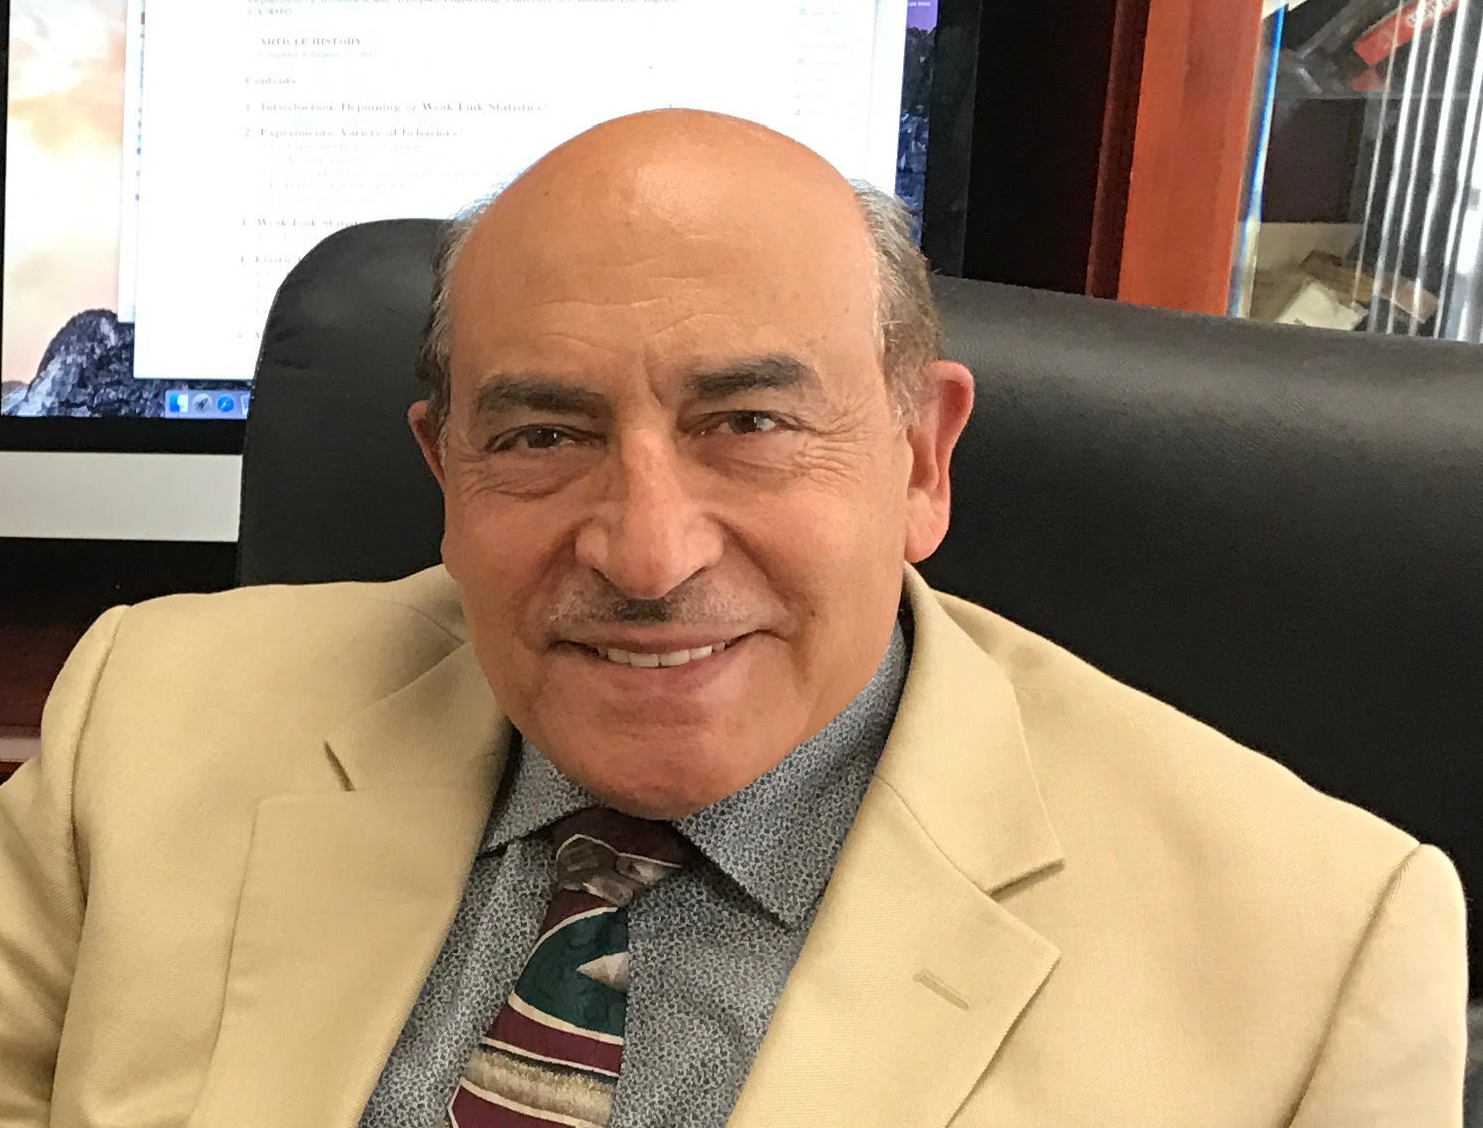
\includegraphics[width=0.4\textwidth]{Nasr-Pic}
\end{wrapfigure}

He was the general chair of the Second International Multiscale Materials Modeling Conference in 2004 and the chair of the 19$^{th}$ International Conference on Fusion Reactor Materials in 2019.  He serves on the editorial boards of several journals and has published over 350 articles, 10 edited books, and is the coauthor of a two-volume book (Oxford Press) on the mechanics and physics of defects, computational materials science, radiation interaction with materials, instabilities, and self-organization in nonequilibrium materials (Oxford Press, 2007, 1100 pages.)  He supervised the graduation of 43 Ph.D. students and 25 postdoctoral scholars. 16 of his former students and postdocs are currently professors in various universities around the world, and many of his former students are technology leaders in the United States. 
\section{Course Overview and Objectives}
The Renewable Energy course provides introductory-level tutorials on the 
conversion principles and technologies in various clean energy sources, such as solar, wind, hydro, biomass, and geothermal. We examine the issues involved in the thermodynamics, design, and operation of three main systems: solar, biomass, and hydro-power. We also discuss the integration of various clean energy sources and their economics. The project is dedicated to enhancing the research experience of students, where three or more groups will conduct independent research under my supervision. At the completion of this course, you will be able to:
\begin{itemize}
    \item Understand the principles of operation of several clean energy technologies.
    \item Analyze the "system" aspects of clean energy technologies.
     \item Realize the technical and economic challenges of each system.
    \item Learn the fundamental principles of thermodynamic energy conversion.
    \item Learn research tools and write a report on the design, operation, integration, or economics of a selected system.
\end{itemize}


Students are expected to spend 120 minutes every two weeks with the instructor and an additional 1-2 hours per week on research and code development.

\textbf{Research Project}: A team project will require students to work together on a feasibility study for a renewable energy development project at a location of their choice using the technologies and tools presented in this class. More details will be provided during the course. The TA will direct the project and the students are expected to make a final presentation. The professor will give short tutorials on research methodology and tools.  These will include Excel or Google Sheets or Python code programming (optional), writing a good research paper using Microsoft Word, Overleaf, or other latex typesetting software for professional report writing, and using Google Scholar and ChatGPT as research assistants.

\newpage

\section{Grading}
	
	\begin{table}[h!]
	    \centering
	    \begin{tabular}{|l|l|}
	         	\hline\hline
	Letter Grade	& Percentage		\\
		\hline\hline  
		A+	& $>$95\%	\\
		A	& 90-95\%	\\
		A-	& 85-90\%	\\
		B+	& 80-85\%	\\
		B & 75-80\%\\
		B-& 70-75\%\\
		C&$<70\%$\\
		\hline\hline
	    \end{tabular}
	    \caption{Letter grade percentages}
	    \label{tab:grades2}
	\end{table}
	
	\newpage
    \section{Research Projects}
\subsection{Photovoltaic Solar Cell Technology}

Silicon-based solar cell technology is a cornerstone of modern renewable energy systems, providing an efficient and sustainable means to harness solar energy. This project invites undergraduate students to explore the key principles and applications of silicon photovoltaics. Students will gain insights into the photoelectric effect, bandgap energy, and spectral absorption properties that underlie the conversion of sunlight into electricity. 

The project will also explore the manufacturing processes of silicon solar cells, examining techniques such as wafer production, doping, and anti-reflective coatings. A focus will be placed on evaluating efficiency improvements through advanced designs like passivated emitter rear contact (PERC) cells.

Beyond theoretical knowledge, students will use Python to simulate the Shockley-Queisser efficiency limit for silicon-based cells. The simulator will allow them to calculate and visualize the efficiency as a function of material properties and environmental conditions. The results will include solar spectrum utilization and recommendations for optimizing cell designs.

The project further explores the economic and environmental implications of solar technology, including cost trends, government incentives, and lifecycle emissions. By the end of the project, students will have a comprehensive understanding of silicon-based solar cell technology and its pivotal role in the transition to sustainable energy systems.
\subsubsection*{Grading Rubric for Solar Project}

\textbf{Total Points: 100}\\
The classification is divided into \textbf{Project Report (70 points)} and \textbf{Final Presentation (30 points)}.

\subsubsection*{1. Project Report (70 points)}
The report will be evaluated based on the following components:

\subsubsection*{A. Review of the literature (15 points)}
\begin{itemize}
    \item \textbf{Comprehensiveness (10 points)}:
    \begin{itemize}
        \item Covers key topics: principles of photovoltaics, spectral absorption, and advanced designs.
        \item Properly cites credible references.
    \end{itemize}
    \item \textbf{Clarity and Structure (5 points)}:
    \begin{itemize}
        \item Written clearly and logically with well-organized sections.
    \end{itemize}
\end{itemize}

\subsubsection*{B. Manufacturing processes (15 points)}
\begin{itemize}
    \item \textbf{Detail and Accuracy (10 points)}:
    \begin{itemize}
        \item Includes detailed descriptions of key manufacturing steps.
        \item Explains their impact on efficiency and cost.
    \end{itemize}
    \item \textbf{Presentation of Data (5 points)}:
    \begin{itemize}
        \item Data are well organized using tables, graphs, or illustrations.
    \end{itemize}
\end{itemize}

\subsubsection*{C. Physics of Solar Photovoltaics (20 points)}
\begin{itemize}
    \item \textbf{Solid state physics principles (10 points)}:
    \begin{itemize}
        \item Silicon-based photovoltaic devices.
        \item Thin films and multijunctions.
    \end{itemize}
    \item \textbf{Testing of solar cells (5 points)}:
    \begin{itemize}
        \item Provides a clear understanding of the solar spectrum conditions for testing the efficiency.
    \end{itemize}
    \item \textbf{Grid-connected solar cells (5 points)}:
    \begin{itemize}
        \item Provides an understanding of the components needed to connect solar cells to the electric grid.
    \end{itemize}
\end{itemize}

\subsubsection*{D. Economic and Environmental Analysis (10 points)}
\begin{itemize}
    \item \textbf{Economic Feasibility (5 points)}:
    \begin{itemize}
        \item Provides detailed calculations for cost trends and incentives.
    \end{itemize}
    \item \textbf{Environmental Impact (5 points)}:
    \begin{itemize}
        \item Addresses life-cycle emissions and sustainability factors.
    \end{itemize}
\end{itemize}

\subsubsection*{E. Report Quality (5 points)}
\begin{itemize}
    \item \textbf{Organization and Flow (3 points)}:
    \begin{itemize}
        \item Sections follow a logical order and are interconnected.
    \end{itemize}
    \item \textbf{Grammar, Style, and Formatting (2 points)}:
    \begin{itemize}
        \item Free of major grammatical errors and formatted consistently.
    \end{itemize}
\end{itemize}

\subsubsection*{F. Extra Credit: Python Code and Simulation (20 points)}
\begin{itemize}
    \item \textbf{Correctness (10 points)}:
    \begin{itemize}
        \item The code executes without errors.
        \item The results align with the theoretical predictions of the Shockley-Queisser limit.
    \end{itemize}
    \item \textbf{Visualization and Insights (5 points)}:
    \begin{itemize}
        \item Provides clear and meaningful graphs of the simulation results.
    \end{itemize}
    \item \textbf{Documentation and Clarity (5 points)}:
    \begin{itemize}
        \item The code is well-documented with comments explaining logic.
    \end{itemize}
\end{itemize}

\subsubsection*{2. Final presentation (30 points)}
The presentation will be evaluated based on the following components:

\subsubsection*{A. Delivery and communication (10 points)}
\begin{itemize}
    \item \textbf{Clarity and Confidence (5 points)}:
    \begin{itemize}
        \item Speakers demonstrate a clear understanding of the project.
        \item Ideas are communicated confidently and concisely.
    \end{itemize}
    \item \textbf{Audience Engagement (5 points)}:
    \begin{itemize}
        \item Visual aids (slides) are effective and engaging.
        \item The team responds effectively to the questions.
    \end{itemize}
\end{itemize}

\subsubsection*{B. Content Coverage (15 points)}
\begin{itemize}
    \item \textbf{Introduction and Objectives (5 points)}:
    \begin{itemize}
        \item Clearly outlines the project objectives and significance.
    \end{itemize}
    \item \textbf{Results and Analysis (5 points)}:
    \begin{itemize}
        \item Key findings, including efficiency simulation results and economic analysis, are presented with graphs or charts.
    \end{itemize}
    \item \textbf{Conclusion and Recommendations (5 points)}:
    \begin{itemize}
        \item Summarizes findings and provides actionable insights.
    \end{itemize}
\end{itemize}

\subsubsection*{C. Time management (5 points)}
\begin{itemize}
    \item The presentation is delivered in the allotted time.
\end{itemize}
\newpage
\subsubsection*{Grading Summary}
\begin{table}[h!]
    \centering
    \begin{tabular}{|l|c|}
        \hline
        \textbf{Category} & \textbf{Points} \\
        \hline
        \textbf{Project Report} & \textbf{70} \\
        Literature Review & 15 \\
        Manufacturing Processes & 15 \\
        Solar Cell Physics & 25 \\
        Economic and Environmental Analysis & 10 \\
        Report Quality & 5 \\
        \hline
        \textbf{Final Presentation} & \textbf{25} \\
        Delivery and Communication & 10 \\
        Content Coverage & 10 \\
        Time Management & 5 \\
        \hline
        \textbf{Total} & \textbf{100} \\
        \hline
         Extra credit - Python Code and Simulation & 20 \\
         \hline
    \end{tabular}
    \caption{Grading Rubric for Silicon-Based Solar Cell Project}
\end{table}

\newpage
\subsection{The Organic Rankine Cycle in Renewable Energy}

The organic Rankine Cycle (ORC) is a crucial technology in the renewable energy sector, offering a pathway to harness low-grade heat sources for sustainable power generation. This undergraduate project focuses on understanding and simulating the ORC, emphasizing its thermodynamic principles, applications, and environmental benefits. Students will explore the selection of organic working fluids, analyze real-world applications such as geothermal and solar power plants, and evaluate the economic feasibility of ORC systems. 

A significant component of the project involves programming in Python to calculate thermodynamic properties, visualize T-S and H-S diagrams, and determine efficiency and power flows using tools like CoolProp. In addition, students will examine the environmental impacts of ORCs, discussing their role in reducing greenhouse gas emissions and using waste heat effectively.

The project integrates theoretical knowledge with practical skills, allowing students to analyze and model energy systems while considering economic and environmental factors. By the end of this project, participants will have a comprehensive understanding of ORC technology and its pivotal role in the advancement of renewable energy solutions. 
\subsubsection*{Grading Rubric for ORC project}

\textbf{Total Points: 100}\\
The classification is divided into \textbf{Project Report (70 points)} and \textbf{Final Presentation (30 points)}.

\subsubsection*{1. Project Report (70 points)}
The report will be evaluated based on the following components:

\subsubsection*{A. Review of the literature (15 points)}
\begin{itemize}
    \item \textbf{Comprehensiveness (10 points)}:
    \begin{itemize}
        \item Covers key topics: ORC principles, fluid selection, and real-world applications.
        \item Properly cites credible references.
    \end{itemize}
    \item \textbf{Clarity and Structure (5 points)}:
    \begin{itemize}
        \item Written clearly and logically with well-organized sections.
    \end{itemize}
\end{itemize}

\subsubsection*{B. Thermodynamic Analysis \& Design (20 points)}
\begin{itemize}
    \item \textbf{Analysis of an Organic Rankine Cycle (10 points)}:
    \begin{itemize}
         \item Statement of the application (e.g. geothermal, OTEC, etc.)
        \item Selection of the appropriate fluid for the application.
        \item Thermodynamic data for the selected fluid.
    \end{itemize}
    \item \textbf{Power Flow in the Cycle (5 points)}:
    \begin{itemize}
         \item Step-by-step results for the power flow in the cycle.
          \item Calculations of heat addition, heat rejection, turbine work, and pump work.
    \end{itemize}
    \item \textbf{Thermodynamic Efficiency (5 points)}:
    \begin{itemize}
        \item Calculations of the thermodynamic efficiency.
        \item Iterations to improve efficiency.
    \end{itemize}
\end{itemize}

\subsubsection*{C. Economic feasibility (15 points)}
\begin{itemize}
    \item \textbf{Detail and Accuracy (10 points)}:
    \begin{itemize}
        \item Includes detailed cost-benefit analysis.
        \item Explains economic feasibility based on payback period and energy cost savings.
    \end{itemize}
    \item \textbf{Clarity (5 points)}:
    \begin{itemize}
        \item Results are presented clearly, using tables or graphs, where appropriate.
    \end{itemize}
\end{itemize}

\subsubsection*{D. Environmental Analysis (10 points)}
\begin{itemize}
    \item \textbf{Impact Assessment (5 points)}:
    \begin{itemize}
        \item Effectively evaluates greenhouse gas emission reductions.
    \end{itemize}
    \item \textbf{Sustainability Insights (5 points)}:
    \begin{itemize}
        \item The purpose of this paper is to discuss the role of ORCs in sustainable energy systems.
    \end{itemize}
\end{itemize}

\subsubsection*{E. Report Quality (10 points)}
\begin{itemize}
    \item \textbf{Organization and Flow (5 points)}:
    \begin{itemize}
        \item The sections follow a logical order and are interconnected.
    \end{itemize}
    \item \textbf{Grammar, Style, and Formatting (5 points)}:
    \begin{itemize}
        \item Free of major grammatical errors and formatted consistently.
    \end{itemize}
\end{itemize}
\subsubsection*{F. Extra Credit -Thermodynamic Simulation (20 points)}
\begin{itemize}
    \item \textbf{Correctness (10 points)}:
    \begin{itemize}
        \item The code executes without errors and produces accurate results.
        \item The results align with the thermodynamic principles.
    \end{itemize}
    \item \textbf{Visualization and Insights (5 points)}:
    \begin{itemize}
        \item Provides clear and meaningful graphs of the T-S and H-S diagrams.
    \end{itemize}
    \item \textbf{Documentation and Clarity (5 points)}:
    \begin{itemize}
        \item The code is well-documented with comments explaining logic.
    \end{itemize}
\end{itemize}

\subsubsection*{2. Final presentation (30 points)}
The presentation will be evaluated based on the following components:

\subsubsection*{A. Delivery and communication (10 points)}
\begin{itemize}
    \item \textbf{Clarity and Confidence (5 points)}:
    \begin{itemize}
        \item Speakers demonstrate a clear understanding of the project.
        \item Ideas are communicated confidently and concisely.
    \end{itemize}
    \item \textbf{Audience Engagement (5 points)}:
    \begin{itemize}
        \item Visual aids (slides) are effective and engaging.
        \item The team responds effectively to the questions.
    \end{itemize}
\end{itemize}

\subsubsection*{B. Content Coverage (15 points)}
\begin{itemize}
    \item \textbf{Introduction and Objectives (5 points)}:
    \begin{itemize}
        \item Clearly outlines the project objectives and significance.
    \end{itemize}
    \item \textbf{Results and Analysis (5 points)}:
    \begin{itemize}
        \item Key findings, including thermodynamic simulations and economic analysis, are presented in graphs or charts.
    \end{itemize}
    \item \textbf{Conclusion and Recommendations (5 points)}:
    \begin{itemize}
        \item Summarizes findings and provides actionable insights.
    \end{itemize}
\end{itemize}

\subsubsection*{C. Time management (5 points)}
\begin{itemize}
    \item The presentation is delivered in the allotted time.
\end{itemize}

\newpage
\subsubsection*{Grading Summary}
\begin{table}[h!]
    \centering
    \begin{tabular}{|l|c|}
        \hline
        \textbf{Category} & \textbf{Points} \\
        \hline
        \textbf{Project Report} & \textbf{70} \\
        Literature Review & 15 \\
        Thermodynamic Analysis and Cycle Design & 25 \\
        Economic Feasibility & 15 \\
        Environmental Analysis & 10 \\
        Report Quality & 10 \\
        \hline
        \textbf{Final Presentation} & \textbf{25} \\
        Delivery and Communication & 10 \\
        Content Coverage & 10 \\
        Time Management & 5 \\
        \hline
        \textbf{Total} & \textbf{100} \\
        \hline
        Extra Credit - Python code for cycle analysis&20\\
        \hline
    \end{tabular}
    \caption{Grading Rubric for Organic Rankine Cycle (ORC) Project}
\end{table}
\newpage
\subsection{Design of a Hydro Power Plant}

Hydropower remains one of the most reliable and sustainable forms of renewable energy, offering opportunities for small-scale applications to supplement local energy demands. This project focuses on the design and analysis of a small-scale hydroelectric power plant using Python-based simulations. Students will begin with a review of the literature to understand the principles of hydropower, including types of plants, turbine technologies, and their environmental and economic implications.

The project progresses to site analysis, where students evaluate key parameters such as river flow rates, head, and seasonal variability. Using a Python code base, they will simulate plant performance, calculate power output, and analyze economic feasibility, including capital costs, annual revenue, and payback periods. Seasonal variations in flow will also be modeled to ensure a robust design.

In addition, students will compare their proposed design with real-world case studies, highlighting the trade-offs between efficiency, cost, and environmental impact. The project ends with a detailed report and presentation summarizing the methodology, results, and recommendations.

This project equips students with practical skills in engineering analysis and design of renewable energy systems, fostering an understanding of sustainable development in the energy sector.


\subsubsection*{Grading Rubric for Hydropower Project}

\textbf{Total Points: 100}\\
The grading is divided into \textbf{Project Report (70 points)} and \textbf{Final Presentation (30 points)}.

\subsubsection*{1. Project Report (70 points)}
The report will be evaluated based on the following components:

\subsubsection*{A. Review of the literature (15 points)}
\begin{itemize}
    \item \textbf{Comprehensiveness (10 points)}:
    \begin{itemize}
        \item Covers key topics: types of hydropower plant, turbines, and environmental/economic impacts.
        \item Properly cites credible references.
    \end{itemize}
    \item \textbf{Clarity and Structure (5 points)}:
    \begin{itemize}
        \item Written clearly and logically with well-organized sections.
    \end{itemize}
\end{itemize}

\subsubsection*{B. Site Analysis (15 points)}
\begin{itemize}
    \item \textbf{Data Quality (10 points)}:
    \begin{itemize}
        \item Includes relevant site-specific parameters (head, flow rate, seasonal variations).
        \item Provides a rationale for turbine selection with respect to technical specifications.
    \end{itemize}
    \item \textbf{Presentation of Data (5 points)}:
    \begin{itemize}
        \item Data is well-organized using tables, graphs, or charts.
    \end{itemize}
\end{itemize}

\subsubsection*{C. Hydroelectric Plant Performance Evaluation}
\begin{itemize}
     \item \textbf{Fundamental Principles of Hydro Power (10 points)}:
    \begin{itemize}
        \item Equations that describe the relationships between flow rate, head, and power.
    \end{itemize}
    \item \textbf{Power Calculations(10 points)}:
    \begin{itemize}
        \item Selection of flow and head parameters.
        \item Calculations of Power Output.
        \item Turbine Selection.
        \item Calculations of the head and flow rate for a selected turbine.
    \end{itemize}
\end{itemize}

\subsubsection*{D. Economic and Environmental Analysis (10 points)}
\begin{itemize}
    \item \textbf{Economic Viability (5 points)}:
    \begin{itemize}
        \item Provides detailed calculations for capital cost, revenue, and repayment period.
    \end{itemize}
    \item \textbf{Environmental Impact (5 points)}:
    \begin{itemize}
        \item Addresses potential environmental trade-offs or sustainability factors.
    \end{itemize}
\end{itemize}

\subsubsection*{E. Comparative analysis (5 points)}
\begin{itemize}
    \item \textbf{Depth of Comparison (3 points)}:
    \begin{itemize}
        \item Effectively compares the design with a real-world case study or benchmarks.
    \end{itemize}
    \item \textbf{Insights and Recommendations (2 points)}:
    \begin{itemize}
        \item Provides meaningful conclusions based on the comparison.
    \end{itemize}
\end{itemize}

\subsubsection*{F. Report Quality (5 points)}
\begin{itemize}
    \item \textbf{Organization and Flow (3 points)}:
    \begin{itemize}
        \item Sections follow a logical order and are interconnected.
    \end{itemize}
    \item \textbf{Grammar, Style, and Formatting (2 points)}:
    \begin{itemize}
        \item Free of major grammatical errors and formatted consistently.
    \end{itemize}
\end{itemize}

\subsubsection*{2. Final presentation (30 points)}
The presentation will be evaluated based on the following components:

\subsubsection*{A. Delivery and communication (10 points)}
\begin{itemize}
    \item \textbf{Clarity and Confidence (5 points)}:
    \begin{itemize}
        \item Speakers demonstrate a clear understanding of the project.
        \item Ideas are communicated confidently and concisely.
    \end{itemize}
    \item \textbf{Audience Engagement (5 points)}:
    \begin{itemize}
        \item Visual aids (slides) are effective and engaging.
        \item The team responds effectively to the questions.
    \end{itemize}
\end{itemize}

\subsubsection*{B. Content Coverage (15 points)}
\begin{itemize}
    \item \textbf{Introduction and Objectives (5 points)}:
    \begin{itemize}
        \item Clearly outlines the project objectives and significance.
    \end{itemize}
    \item \textbf{Results and Analysis (5 points)}:
    \begin{itemize}
        \item Key findings, including power output, economic analysis, and seasonal variability, are presented with graphs or charts.
    \end{itemize}
    \item \textbf{Conclusion and Recommendations (5 points)}:
    \begin{itemize}
        \item Summarizes findings and provides actionable insights.
    \end{itemize}
\end{itemize}

\subsubsection*{C. Time management (5 points)}
\begin{itemize}
    \item The presentation is delivered in the allotted time.
\end{itemize}

\subsubsection*{Grading Summary}
\begin{table}[h!]
    \centering
    \begin{tabular}{|l|c|}
        \hline
        \textbf{Category} & \textbf{Points} \\
        \hline
        \textbf{Project Report} & \textbf{70} \\
        Literature Review & 15 \\
        Site Analysis & 15 \\
        Hydroelectric Plant Performance Evaluation& 25 \\
        Economic and Environmental Analysis & 10 \\
        Comparative Analysis & 5 \\
        Report Quality & 5 \\
        \hline
        \textbf{Final Presentation} & \textbf{25} \\
        Delivery and Communication & 10 \\
        Content Coverage & 10 \\
        Time Management & 5 \\
        \hline
        \textbf{Total} & \textbf{100} \\
        \hline
    \end{tabular}
    \caption{Grading Rubric for Hydropower Project}
\end{table}
\newpage 

\subsection{Wind Energy: Design and Environmental Impact}

\subsubsection*{Overview}

Wind energy is a key renewable energy technology that uses the kinetic energy of the wind to generate electricity. This project aims to explore the principles, technology and implementation of wind turbines, as well as their economic and environmental impacts. Students will gain a deep understanding of wind energy systems, from historical milestones to cutting-edge technologies like offshore wind farms.

\subsubsection*{Objectives}

By the end of this project, students will be able to:

\begin{enumerate}
    \item Analyze the historical development of wind energy and its current penetration in the global market.
    \item Understand the physics of wind turbine operation, including concepts like lift, drag, and Betz's limit.
    \item Examine the design principles of modern wind turbines, focusing on components such as rotor blades, alternators, and control systems.
    \item Investigate environmental and economic impacts, assessing greenhouse gas reductions and cost-benefit analyses.
    \item Perform simplified calculations to evaluate performance metrics using spreadsheet tools like Microsoft Excel or Google Sheets.
\end{enumerate}

\subsubsection*{Project Components}

\begin{enumerate}
    \item \textbf{Literature Review (10 Points):}
    \begin{itemize}
        \item Comprehensive study of the history of wind energy, technological advancements, and trends of global adoption.
        \item The sources must be properly cited.
    \end{itemize}

    \item \textbf{Physics and Design of Wind Turbines (20 Points):}
    \begin{itemize}
        \item Analysis of lift and drag forces and their role in turbine efficiency.
        \item Explanation of Betz's limit and its practical implications.
        \item Exploration of turbine components (e.g., rotor blades, hubs, and generators).
    \end{itemize}

    \item \textbf{Performance Evaluation using Simplified Calculations (20 Points):}
    \begin{itemize}
        \item Use spreadsheet tools to model turbine performance.
        \item Create tables and charts to visualize power output at various wind speeds.
        \item Analyze the effects of blade length, rotor diameter, and hub height.
    \end{itemize}

    \item \textbf{Environmental and Economic Analysis (15 Points):}
    \begin{itemize}
        \item Quantification of reductions in the carbon footprint.
        \item Cost analysis, including installation, maintenance, and lifecycle costs.
    \end{itemize}

    \item \textbf{Comparative Study (10 Points):}
    \begin{itemize}
        \item Comparison of onshore and offshore wind systems.
        \item Case studies of successful wind farms worldwide.
    \end{itemize}

    \item \textbf{Final Report and Presentation (25 Points):}
    \begin{itemize}
        \item Comprehensive documentation of findings.
        \item Effective communication of results through charts, graphs, and a structured narrative.
        \item The presentation must engage the audience and adhere to time constraints.
    \end{itemize}
\end{enumerate}

\subsubsection*{Tools and Resources}

Students will use resources such as scientific journals, spreadsheet tools (e.g., Microsoft Excel or Google Sheets), and case studies to complete the project. Guidance on data visualization and calculations will be provided during the course.

\subsubsection*{Grading Rubric}

\begin{center}
\begin{tabular}{|l|c|}
\hline
\textbf{Category} & \textbf{Points} \\
\hline
\textbf{Project Report} & \textbf{70} \\
Literature Review & 10 \\
Physics and Design Analysis & 20 \\
Performance Evaluation & 20 \\
Environmental and Economic Impact & 15 \\
Comparative Study & 10 \\
 \hline
        \textbf{Final Presentation} & \textbf{25} \\
        Delivery and Communication & 10 \\
        Content Coverage & 10 \\
        Time Management & 5 \\
        \hline
\hline
\textbf{Total} & \textbf{100} \\
\hline
\end{tabular}
\end{center}

This project combines theoretical knowledge with practical skills, equipping students to analyze, model, and optimize wind energy systems. By integrating environmental and economic perspectives, students will also understand the broader implications of renewable energy technologies in combating climate change.


\subsection{Tidal Energy Technologies}

\subsubsection*{Overview}
Tidal energy is a promising renewable energy technology that utilizes the kinetic and potential energy of tidal movements to generate electricity. This project explores various tidal energy systems, including barrages, lagoons, and tidal stream turbines, focusing on their principles, design, and environmental and economic impacts.

\subsubsection*{Objectives}
By the end of this project, students will:
\begin{enumerate}
    \item Understand the physical principles behind the generation of tidal energy.
    \item Examine the design and operation of tidal energy systems, such as barrages and tidal stream turbines.
    \item Evaluate the environmental and economic impacts of tidal energy systems.
    \item Perform simplified performance evaluations using spreadsheet tools (for example, Microsoft Excel or Google Sheets).
\end{enumerate}

\subsubsection*{Project Components}
\begin{enumerate}
    \item \textbf{Literature Review (10 Points):}
    \begin{itemize}
        \item Study the history and development of tidal energy technologies.
        \item Analyze the adoption and challenges of tidal energy worldwide.
    \end{itemize}

    \item \textbf{Physics and Design of Tidal Systems (20 Points):}
    \begin{itemize}
        \item Explore the principles of operation of tidal barrages, lagoons, and stream turbines.
        \item Use simplified equations to calculate potential energy and power output.
    \end{itemize}

    \item \textbf{Performance Evaluation using Spreadsheets (20 Points):}
    \begin{itemize}
        \item Create tables to calculate energy output based on tidal ranges, water density, and turbine efficiency.
        \item Use charts to visualize energy output across different tidal cycles.
        \item Perform a sensitivity analysis to understand the impact of key parameters (e.g., turbine efficiency, tidal range).
    \end{itemize}

    \item \textbf{Environmental and Economic Analysis (15 Points):}
    \begin{itemize}
        \item Assess environmental benefits, such as reduced greenhouse gas emissions.
        \item Evaluate possible ecological disruptions and mitigation strategies.
        \item Perform a cost-benefit analysis, focusing on capital and maintenance costs.
    \end{itemize}

    \item \textbf{Comparative Study (10 Points):}
    \begin{itemize}
        \item Compare tidal energy with other renewable energy sources (e.g., wind, solar).
        \item Highlight advantages and limitations of tidal energy systems.
    \end{itemize}

    \item \textbf{Final Report and Presentation (25 Points):}
    \begin{itemize}
        \item Document findings in a detailed report with visuals and charts.
        \item Present results in a clear and engaging manner.
    \end{itemize}
\end{enumerate}

\subsubsection*{Tools and Resources}
Students will use resources such as scientific journals, technical reports, and spreadsheet tools (e.g., Microsoft Excel or Google Sheets) to perform calculations and analyze data. Templates and guidance on spreadsheet use will be provided during the course.

\subsubsection*{Grading Rubric}
\begin{center}
\begin{tabular}{|l|c|}
\hline
\textbf{Category} & \textbf{Points} \\
\hline
\textbf{Project Report} & \textbf{70} \\
Literature Review & 10 \\
Physics and Design Analysis & 20 \\
Performance Evaluation & 20 \\
Environmental and Economic Impact & 15 \\
Comparative Study & 10 \\
 \hline
        \textbf{Final Presentation} & \textbf{25} \\
        Delivery and Communication & 10 \\
        Content Coverage & 10 \\
        Time Management & 5 \\
        \hline
\hline
\textbf{Total} & \textbf{100} \\
\hline
\end{tabular}
\end{center}

This project aims to combine theoretical understanding with practical skills, equipping students to critically evaluate and optimize tidal energy systems. By integrating environmental and economic considerations, students will understand the broader implications of adopting renewable energy technologies.
\newpage
\subsection{Deep Geothermal Energy: Physical Principles and Technology Evaluation}

\subsubsection*{Overview}
Deep geothermal energy is a renewable energy source that utilizes the heat stored beneath the Earth's surface for electricity generation and heating applications. This project explores the physical principles, current technology, implementation methods, economic viability, and environmental impact of deep geothermal energy systems.

\subsubsection*{Objectives}
By the end of this project, students will:
\begin{enumerate}
    \item Understand the physical principles governing geothermal energy extraction.
    \item Explore current technologies for geothermal energy production, including dry steam and binary cycle systems.
    \item Evaluate environmental and economic impacts of geothermal energy systems.
    \item Perform simplified calculations using spreadsheet tools (e.g. Microsoft Excel or Google Sheets) to model geothermal system performance.
\end{enumerate}

\subsubsection*{Project Components}
\begin{enumerate}
    \item \textbf{Literature Review (10 Points):}
    \begin{itemize}
        \item Study the history and evolution of deep geothermal energy technologies.
        \item Summarize the challenges and advancements in the field.
    \end{itemize}

    \item \textbf{Physical Principles and Design (20 Points):}
    \begin{itemize}
        \item Understand geothermal heat transfer mechanisms and thermodynamic cycles (e.g., Rankine and Organic Rankine Cycles).
        \item Perform simple energy calculations using spreadsheet tools to evaluate heat extraction rates and energy efficiency.
    \end{itemize}

    \item \textbf{Performance Evaluation using Spreadsheets (20 Points):}
    \begin{itemize}
        \item Create models to calculate power output based on the depth of the well, the temperature of the rock, and the thermal conductivity.
        \item Analyze the effects of different system configurations using tables and charts.
    \end{itemize}

    \item \textbf{Environmental and Economic Impact (15 Points):}
    \begin{itemize}
        \item Assess the benefits, such as the reduction of greenhouse gases, and risks, such as induced seismicity.
        \item Evaluate economic factors such as the levelized cost of energy (LCOE) and the initial investment requirements.
    \end{itemize}

    \item \textbf{Comparative Study (10 Points):}
    \begin{itemize}
        \item Compare geothermal energy with other renewable energy sources.
        \item Highlight advantages, limitations, and potential for integration.
    \end{itemize}

    \item \textbf{Final Report and Presentation (25 Points):}
    \begin{itemize}
        \item Document findings in a well-structured report with visuals and charts.
        \item Present results effectively, focusing on clarity and engagement.
    \end{itemize}
\end{enumerate}

\subsubsection*{Tools and Resources}
Students will use scientific literature, technical reports, and spreadsheet tools (e.g., Microsoft Excel or Google Sheets) for calculations and data visualization. Support for spreadsheet modeling will be provided during the course.

\subsubsection*{Grading Rubric}
\begin{center}
\begin{tabular}{|l|c|}
\hline
\textbf{Category} & \textbf{Points} \\
\hline
\textbf{Project Report} & \textbf{70} \\
Literature Review & 10 \\
Physical Principles and Design & 20 \\
Performance Evaluation & 20 \\
Environmental and Economic Impact & 15 \\
Comparative Study & 10 \\
 \hline
        \textbf{Final Presentation} & \textbf{25} \\
        Delivery and Communication & 10 \\
        Content Coverage & 10 \\
        Time Management & 5 \\
        \hline
\hline
\textbf{Total} & \textbf{100} \\
\hline
\end{tabular}
\end{center}

This project aims to combine theoretical understanding with practical application, enabling students to analyze, model, and evaluate geothermal energy systems in a comprehensive way. The integration of environmental and economic perspectives ensures a holistic approach to renewable energy technology.
\newpage

\subsection{Biofuel Technology: Design Principles, Feedstock Analysis & Environmental Impact}

\subsubsection*{Overview}
Biofuel technology involves the production of renewable fuels from biological feedstocks such as crops, algae and agricultural residues. This project explores the current design principles, the main feedstocks, the environmental impact and future growth of biofuel technology, with a focus on the production of biodiesel and bioethanol.

\subsubsection*{Objectives}
By the end of this project, students will:
\begin{enumerate}
    \item Understand the principles and processes involved in the production of biodiesel and bioethanol.
    \item Analyze the environmental and economic impacts of the production and use of biofuels.
    \item Evaluate the performance of biofuel systems using spreadsheet tools (e.g., Microsoft Excel or Google Sheets).
    \item Explore future growth trends and challenges in the biofuel industry.
\end{enumerate}

\subsubsection*{Project Components}
\begin{enumerate}
    \item \textbf{Literature Review (10 Points):}
    \begin{itemize}
        \item Study the history and development of biofuels, including key milestones.
        \item Summarize current technologies used for biodiesel and bioethanol production.
    \end{itemize}

    \item \textbf{Design Principles and Feedstocks (20 Points):}
    \begin{itemize}
        \item Explore the processes of transesterification for biodiesel and fermentation for bioethanol.
        \item Compare the characteristics of the main feedstocks, such as corn, sugarcane, and algae.
    \end{itemize}

    \item \textbf{Performance Evaluation using Spreadsheets (20 Points):}
    \begin{itemize}
        \item Model the production efficiency of biofuels based on feedstock input, yield rates, and conversion processes.
        \item Create visualizations (charts and graphs) to illustrate trends and efficiencies.
    \end{itemize}

    \item \textbf{Environmental and Economic Impact (15 Points):}
    \begin{itemize}
        \item Assess greenhouse gas reductions, energy payback ratios, and water usage.
        \item Perform cost analysis, including feedstock prices and production costs.
    \end{itemize}

    \item \textbf{Future Growth Analysis (10 Points):}
    \begin{itemize}
        \item Evaluate potential advancements in biofuel technology, including second- and third-generation feedstocks.
        \item Explore challenges such as feedstock availability and scalability.
    \end{itemize}

    \item \textbf{Final Report and Presentation (25 Points):}
    \begin{itemize}
        \item Document the findings in a detailed report with tables, charts, and references.
        \item Present the results effectively, focusing on clarity and participation.
    \end{itemize}
\end{enumerate}

\subsubsection*{Tools and Resources}
Students will use scientific articles, technical reports, and spreadsheet tools (e.g., Microsoft Excel or Google Sheets) to perform calculations and analyze data. Templates and examples will be provided to support spreadsheet modeling.

\subsubsection*{Grading Rubric}
\begin{center}
\begin{tabular}{|l|c|}
\hline
\textbf{Category} & \textbf{Points} \\
\hline
\textbf{Project Report} & \textbf{70} \\
Literature Review & 10 \\
Design Principles and Feedstocks & 20 \\
Performance Evaluation & 20 \\
Environmental and Economic Impact & 15 \\
Future Growth Analysis & 10 \\
 \hline
        \textbf{Final Presentation} & \textbf{25} \\
        Delivery and Communication & 10 \\
        Content Coverage & 10 \\
        Time Management & 5 \\
        \hline
\hline
\textbf{Total} & \textbf{100} \\
\hline
\end{tabular}
\end{center}

The purpose of this project is to combine theoretical understanding with practical skills, enabling students to critically evaluate and optimize biofuel technologies. The integration of environmental and economic analyses ensures a comprehensive approach to renewable energy.
\newpage

\subsection{Wave Energy: Principles, Technology, Environmental and Economic Impact}

\subsubsection*{Overview}
Wave energy harnesses the kinetic and potential energy of ocean waves to generate electricity. This project investigates the historical development, physical principles, implementation technologies, environmental impacts, and future prospects of wave energy systems.

\subsubsection*{Objectives}
By the end of this project, students will:
\begin{enumerate}
    \item Understand the physical principles that govern wave energy conversion.
    \item Explore different wave energy converter (WEC) technologies and their implementations.
    \item Evaluate the environmental and economic impacts of wave energy systems.
    \item Use spreadsheet tools (e.g., Microsoft Excel or Google Sheets) to perform simplified calculations for wave energy system performance.
    \item Examine the future potential and challenges of wave energy development.
\end{enumerate}

\subsubsection*{Project Components}
\begin{enumerate}
    \item \textbf{Literature Review (10 Points):}
    \begin{itemize}
        \item Review the history of wave energy utilization, from early concepts to modern advancements.
        \item We discuss key milestones and the current state of wave energy technologies.
    \end{itemize}

    \item \textbf{Physical Principles and Design (20 Points):}
    \begin{itemize}
        \item Explain how wave energy is derived from the dynamics of the wind and ocean.
        \item Use simplified equations to calculate the wave energy potential, power output, and efficiency.
    \end{itemize}

    \item \textbf{Performance Evaluation using Spreadsheets (20 Points):}
    \begin{itemize}
        \item Model wave energy output based on parameters such as wave height, period, and device efficiency.
        \item Visualize trends and comparisons using tables and charts.
        \item Perform a sensitivity analysis to understand the impact of different variables on performance.
    \end{itemize}

    \item \textbf{Environmental and Economic Impact (15 Points):}
    \begin{itemize}
        \item Assess the effects of wave energy devices on marine ecosystems and coastal environments.
        \item Evaluate the economic feasibility of wave energy systems, including capital and operational costs.
    \end{itemize}

    \item \textbf{Future Prospects (10 Points):}
    \begin{itemize}
        \item Discuss the challenges and opportunities for wave energy in global energy markets.
        \item Explore innovative technologies and their potential to improve efficiency and reduce costs.
    \end{itemize}

    \item \textbf{Final Report and Presentation (25 Points):}
    \begin{itemize}
        \item Prepare a detailed report summarizing findings, supported by tables, charts, and references.
        \item Present the results effectively, emphasizing clarity and engagement.
    \end{itemize}
\end{enumerate}

\subsubsection*{Tools and Resources}
Students will use scientific literature, technical reports, and spreadsheet tools (e.g., Microsoft Excel or Google Sheets) for calculations and data analysis. Templates and guidance for spreadsheet modeling will be provided.

\subsubsection*{Grading Rubric}
\begin{center}
\begin{tabular}{|l|c|}
\hline
\textbf{Category} & \textbf{Points} \\
\hline
\textbf{Project Report} & \textbf{70} \\
Literature Review & 10 \\
Physical Principles and Design & 20 \\
Performance Evaluation & 20 \\
Environmental and Economic Impact & 15 \\
Future Prospects & 10 \\
 \hline
        \textbf{Final Presentation} & \textbf{25} \\
        Delivery and Communication & 10 \\
        Content Coverage & 10 \\
        Time Management & 5 \\
        \hline
\hline
\textbf{Total} & \textbf{100} \\
\hline
\end{tabular}
\end{center}

This project combines theoretical insights with practical evaluation techniques, enabling students to analyze, model, and assess wave energy systems comprehensively. The inclusion of environmental and economic perspectives ensures a holistic understanding of renewable energy technologies.

\end{document}
